\chapter{Imaging Air Cherenkov Astronomy}
\label{ch:iact}
%
\begin{figure}[H]
  \centering
  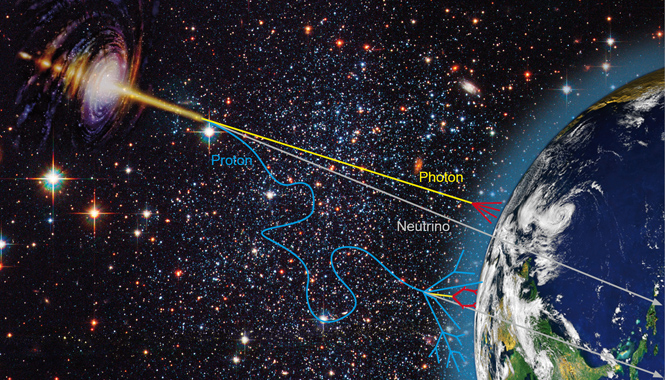
\includegraphics[width=0.95\textwidth]{Plots/cosmic_rays.jpg}
  \caption{Different constituents of the cosmic rays reaching earth \cite{cosmic-rays}. There are three different particle types of cosmic rays that can be used for astronomy. The uncharged and very light neutrinos (white) barely interact with anything on their way through the universe. Thus, they give strong hints on their origin, but are very hard to detect as well. The charged particles such as protons or ionized atoms (blue) are deflected by magnetic fields and therefore lose any direction information. Lastly, cosmic gamma-rays (yellow), massless uncharged photons, are emitted through various processes and from different sources such as active galctic nuclei. They are not deflected much and are the main signal for Cherenkov astronomy.}
  \label{fig:rays}
\end{figure}
%
The atmosphere of earth is continously penetrated by radiation from different
sources within our universe. This cosmic radiation is made up of different types
of particles, interacting with the atmosphere in various ways. There are
charged protons and the uncharged neutrinos and photons (gamma rays). Neutrinos
are uncharged, very light fermions, that interact very weakly and are not
detectable by optical telescopes at all. Protons make up the largest number of
particles reaching earths atmosphere. Due to their electric charge, they are
deflected by magnetic fields and therefore lose information on their origin on
the way to earth, making them unsuitable for Cherenkov astronomy.
%
\section{Cosmic Gamma-Rays}
%
Cosmic gamma-rays are photons with a very high energy, originating from bright
sources such as active galactic nuclei or nebulae. When such particles intersect
with earth's atmosphere, they create new particles moving faster than light
within that atmosphere due to their high energy. Particles moving at such
speeds through a medium cause, among the creation of other particles, the
emission of bluish photons, the Cherenkov-light.
Cherenkov-light is emitted by the medium directly from the moving particle
within a specific angle towards the direction of movement of that primary
particle.
%
\begin{equation}
    \cos(\vartheta) = \frac{1}{n\beta}
    \label{eq:angle_cherenkov}
\end{equation}
%
As \autoref{eq:angle_cherenkov} shows, this angle depends on the index of
refraction $n$ of the medium and the particle's velocity. Due to this emission
angle the light traverses the medium in a cone-shape, when being described from
earth's point of view. By the time it is reaching the ground it thus
illuminates an elliptical area of about $\SI{200}{\meter}$ diameter, depending
on the height of interaction and the primary particle's energy.
This already implicates that the light, although a secondary product of the
cosmic gamma-ray, can be used to reconstruct physical properties of
said gamma-ray. To do so, the flashes of the Cherenkov-light need to
be captured by cameras capable of filming very short time scales (about
$\SI{e-9}{\second}$).

\section{Imaging Air Cherenkov Telescopes}

Imaging Air Cherenkov Telescopes (IACTs) are using videos of this light, to
reconstruct properties of the incident cosmic radiation above
$\SI{100}{\giga\electronvolt}$, by analyzing the spatial geometry of the
measured pictures.
% \newpage

The three properties of interest for each event are:
%
\begin{description}[labelsep=1em, align=right]
  \item[source position]{the position of the source of the primary particle on the sky}
  \item[particle type]{the distinction between cosmic gamma rays and other particles like protons or secondary particles like muons}
  \item[particle energy]{the energy of the primary gamma-ray}
\end{description}
%
This means that the task is to resolve single incoming cosmic gamma rays and
reconstruct these properties. By doing so, the atmosphere is used as a very
wide spread detector. When trying to avoid any interactions of the incident
particles and measuring their properties directly in a specifically prepared
detector material, one eventuually has to leave earth's atmosphere. Such direct
measurements are carried out in earth's orbit, outside its atmosphere.
Detectors like the Fermi Large-Area-Telescope \cite{fermiLAT} (Fermi LAT) are satellites
carrying their own detectors for the necessary measurements. They consist of
interaction volumes taking over what the atmosphere does to intersecting cosmic
rays: particles like gamma rays interact with the material, creating new
particles by losing energy, which then continue to do so in particle cascades
until the energy has spread to a certain amount. This process is called
shower (or air-shower, depending on the medium of interaction). The
characteristics of these interactions and the produced particles strongly
depend on the properties of the incident particle, such as energy and particle
type. There are particles that mainly interact via the electromagnetic force.
Such showers are called electromagnetic showers. They are usually initiated by
photons or electrons and mainly consist of light, charged fermions like electrons or
muons and photons or light, charged bosons like pions. Showers initiated by
hadronic cosmic rays like protons show different kinds of interactions, also
resulting in different spatial topologies. The momentum perpendicular to the
primary particle's trajectory is bigger, giving the shower a wider spread of
secondary particles. This is the main characteristic to distinguish hadronic
showers, resembling the main background within the measurements (apart from
muons) from signal gamma rays. When a proton interacts with a
nucleus within the atmosphere or a dedicated detector material, a lot of
different particles can be created. Heavier hadrons usually quickly decay into
the lightest ones which are protons for the class of baryons as well as pions
for the class of mesons. The pions mainly decay into muons, which eventually
yield electrons and neutrinos. During all those interactions photons and
electrons and their anti-particles as well as neutrinos are created. The
neutrinos very rarely contribute to any interactions after their creation,
whereas electrons can interact with photons, emit or absorb them or annihilate
to such.

\begin{figure}
  \centering
  \begin{subfigure}{0.475\textwidth}
    \centering
    \includegraphics[width=0.85\textwidth]{example-image-a}
    \label{fig:proton}
  \end{subfigure}
  \begin{subfigure}{0.475\textwidth}
    \centering
    \includegraphics[width=0.85\textwidth]{example-image-b}
    \label{fig:gamma}
  \end{subfigure}
  \caption{Simple sketch of the two different shower types.}
  \label{fig:shower}
\end{figure}

Considering this, the higher the energy of the incident particle the more
energy is available for the resulting shower. Thus, the size of these showers
is expected to strongly correlate with the energy. But, to register a cosmic
ray, there has to be interaction first. The effective area of the telescope
is mainly determined by the interactions that can be covered by the sensors. So
bringing up a detector to earth's orbit strongly limits the sensored
interaction material, which already highlights the disadvantage of satellite
telescopes: the amount of interaction material is strongly limited and the
measurement is strongly dependent on that quantity. Direct measurements, e.g.
can derive the direction of cosmic rays by reconstructing the interactions of
the cosmic ray itself inside the tracker volume, rather than secondary
particles. They also give the possibility to measure the energy by counting the
energy depositions within a well calibrated and understood calorimeter, as well
as the particle type. But the strong limitations on size and weight confine the
effective areas of such telescopes very strictly. Thus, detectors in space are
usually unable to resolve time structures of events, but are well suited for
static and wide field-of-view surveys with large exposure times. Since the
abundance of cosmic rays is dependent on the energy and high energy cosmic rays
are much less likely to appear, such detectors are rather suited for the lower
energies.

So there are quite some disadvantages that direct measurements have over
indirect measurements and vice versa. Of course, using the atmosphere means
using a detector undergoing strong, uncontrollable fluctuations in all its
properties. It also means using a detector that is bigger than anything
man-build and readily available. Good understanding of these fluctuations and
the respective modelling is crucial for the analysis of the data.

High energy cosmic particles interacting with the earth's atmosphere generate
showers as described above in a highly boosted way. The secondary particles
therefore continue their trajectories almost parallel to the incident particle.
The spatial distribution of the shower again depends on the energy of the
cosmic ray, ranging from several kilometers to showers not reaching their
climax before hitting the ground. IACTs record the Cherenkov photons of the
showers from energies of about $\SI{100}{\giga\electronvolt}$ to the highest
energies of the cosmic spectrum. But since the cosmic ray energy spectrum
rapidly decreases at high energies, the majority of the recorded events
resemble the lower energy limit of the telescopes.
